% !TEX root = ../Abschlussbericht_Schimmeliger_Keller.tex
%%
%%  Hochschule für Technik und Wirtschaft Berlin --  Projektabschlussbericht
%%
%% Kapitel 4 - Praktische Umsetzung
%%
%%

\chapter{Praktische Umsetzung} \label{Praktische Umsetzung}
\section{Verwendete Hardware} \label{Hardware}
\subsection{LoPy4-Development-Board} \label{LoPy4}

Das LoPy4 ist ein von Pycom Ltd. hergestelltes Development-Board für die Anwendungen im IoT-Bereich. Es unterstützt viele Schnittstellen und Übertragungsprotokolle, die für IoT-Anwendung von großer Relevanz sind. Die Abbildung \ref{fig:lopy-blockschaltbild} stellt die Funktionalitäten des LoPy4-Development-Boards in Form eines Blockdiagrammes  dar. 

\begin{figure}[h]
 \centering
 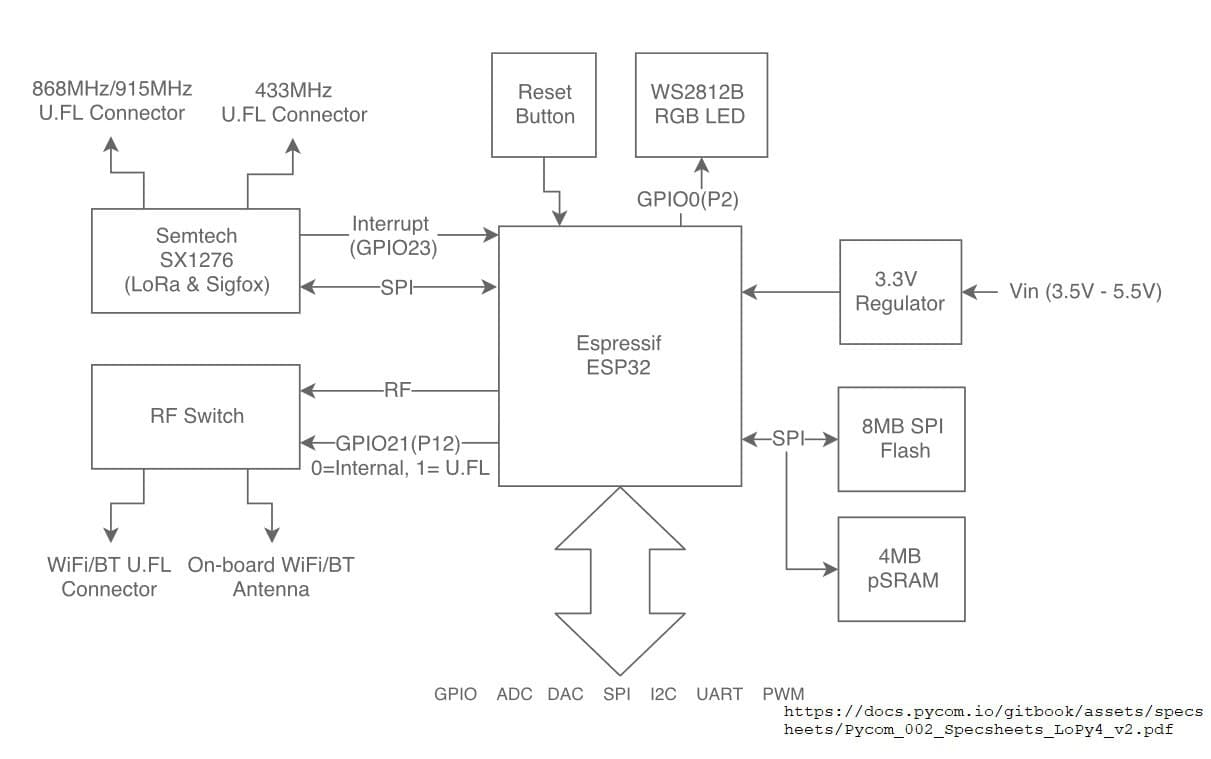
\includegraphics[width=1\textwidth]{pictures/blockdiagram_lopy}
 \caption[LoPy4-Blockdiagramm]{LoPy4-Blockdiagramm}\cite{Lopy2022}
 \label{fig:systemkonzept}
\end{figure}

Im Kern befindet sich ein Espressif ESP32 mit Xtensa dual-core-32-bit LX6 Mikroprozessor. Als Speicher verwendet es 520KB + 4MB RAM und einen externen 8MB Flash-Speicher, wohin auch der Code dann geladen wird. 

Zur Ein-/Ausgabe und der Steuerung von Sensoren und Aktoren, bietet das Board vielseitige Peripherien wie GPIO, ADC, DAC, SPI, I2C, UART und PWM an. 

Darüberhinaus verfügt das Entwicklungsboard über WLAN (802.11b/g/n/e/i), Bluetooth/Bluetooth Low Energy (BLE) v4.2, sowie LoRa und Sigfox Protokolle.  

Es lässt sich leicht mit einem Breadboard benutzen, um damit einfache Schaltungen, ohne zu löten, testen zu können. 

\subsection{DHT Sensormodul} \label{DHT}

\begin{center}
	\begin{figure}[h]
	 
	 \noindent\makebox[\textwidth]{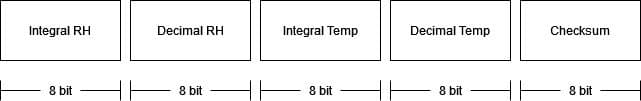
\includegraphics[width=0.7\textwidth]{pictures/dht11_dataframe}}
	 \caption[DHT Paketstruktur]{DHT Paketstruktur}
	 \label{fig:zeitplanung}
	\end{figure}
\end{center}



\subsection{Restliche Hardware} \label{Restliche Hardware}




\section{Beschreibung der Software} \label{Software}

Für unser Projekt haben wir drei verschiedene, miteinander interagierende Software Komponenten realisiert, welche über eine Schnittstelle (Interface) miteinander kommunizieren. 
Der Vorteil einer solchen Architektur ist, dass die einzelnen Komponenten sich unter umständen wiederverwenden lassen und sich im Idealfall so eine Software modular aufbauen lässt.
Da wir als Programmiersprache ausschließlich Python bzw. Micropython verwendet haben, könnte man argumentieren, dass unsere Software automatisch Modular ist, da sich in der Theorie alle programmierten Komponenten in Python wiederverwenden lassen.
Dies ist aber sehr verallgemeinert gesprochen, da gerade die Programmierung der Mikrocontroller definitiv auch Individualsoftware benötigt, welche sich aber immerhin nicht nur auf einer einzelnen Mikrocontrollerfamilie ausführen funktionieren würde.
Anzumerken ist noch, dass für unsere finale Version des Projektes vermutlich nur eine einzelne Softwarekomponente notwendig wäre.


\subsection{1. Komponente: Sensoransteuerung und der Versand der Daten mittels LoRa(WAN)} \label{Sender}

Für die Programmierung der Mikrocontroller verwenden wir die Programmiersprache Micropython, welche eine schlanke und schnelle Implementation der Programmiersprache Python ist, welche für Mikrocontroller optimiert wurde.

\begin{center}
	\begin{figure}[h]
	 
	 \noindent\makebox[\textwidth]{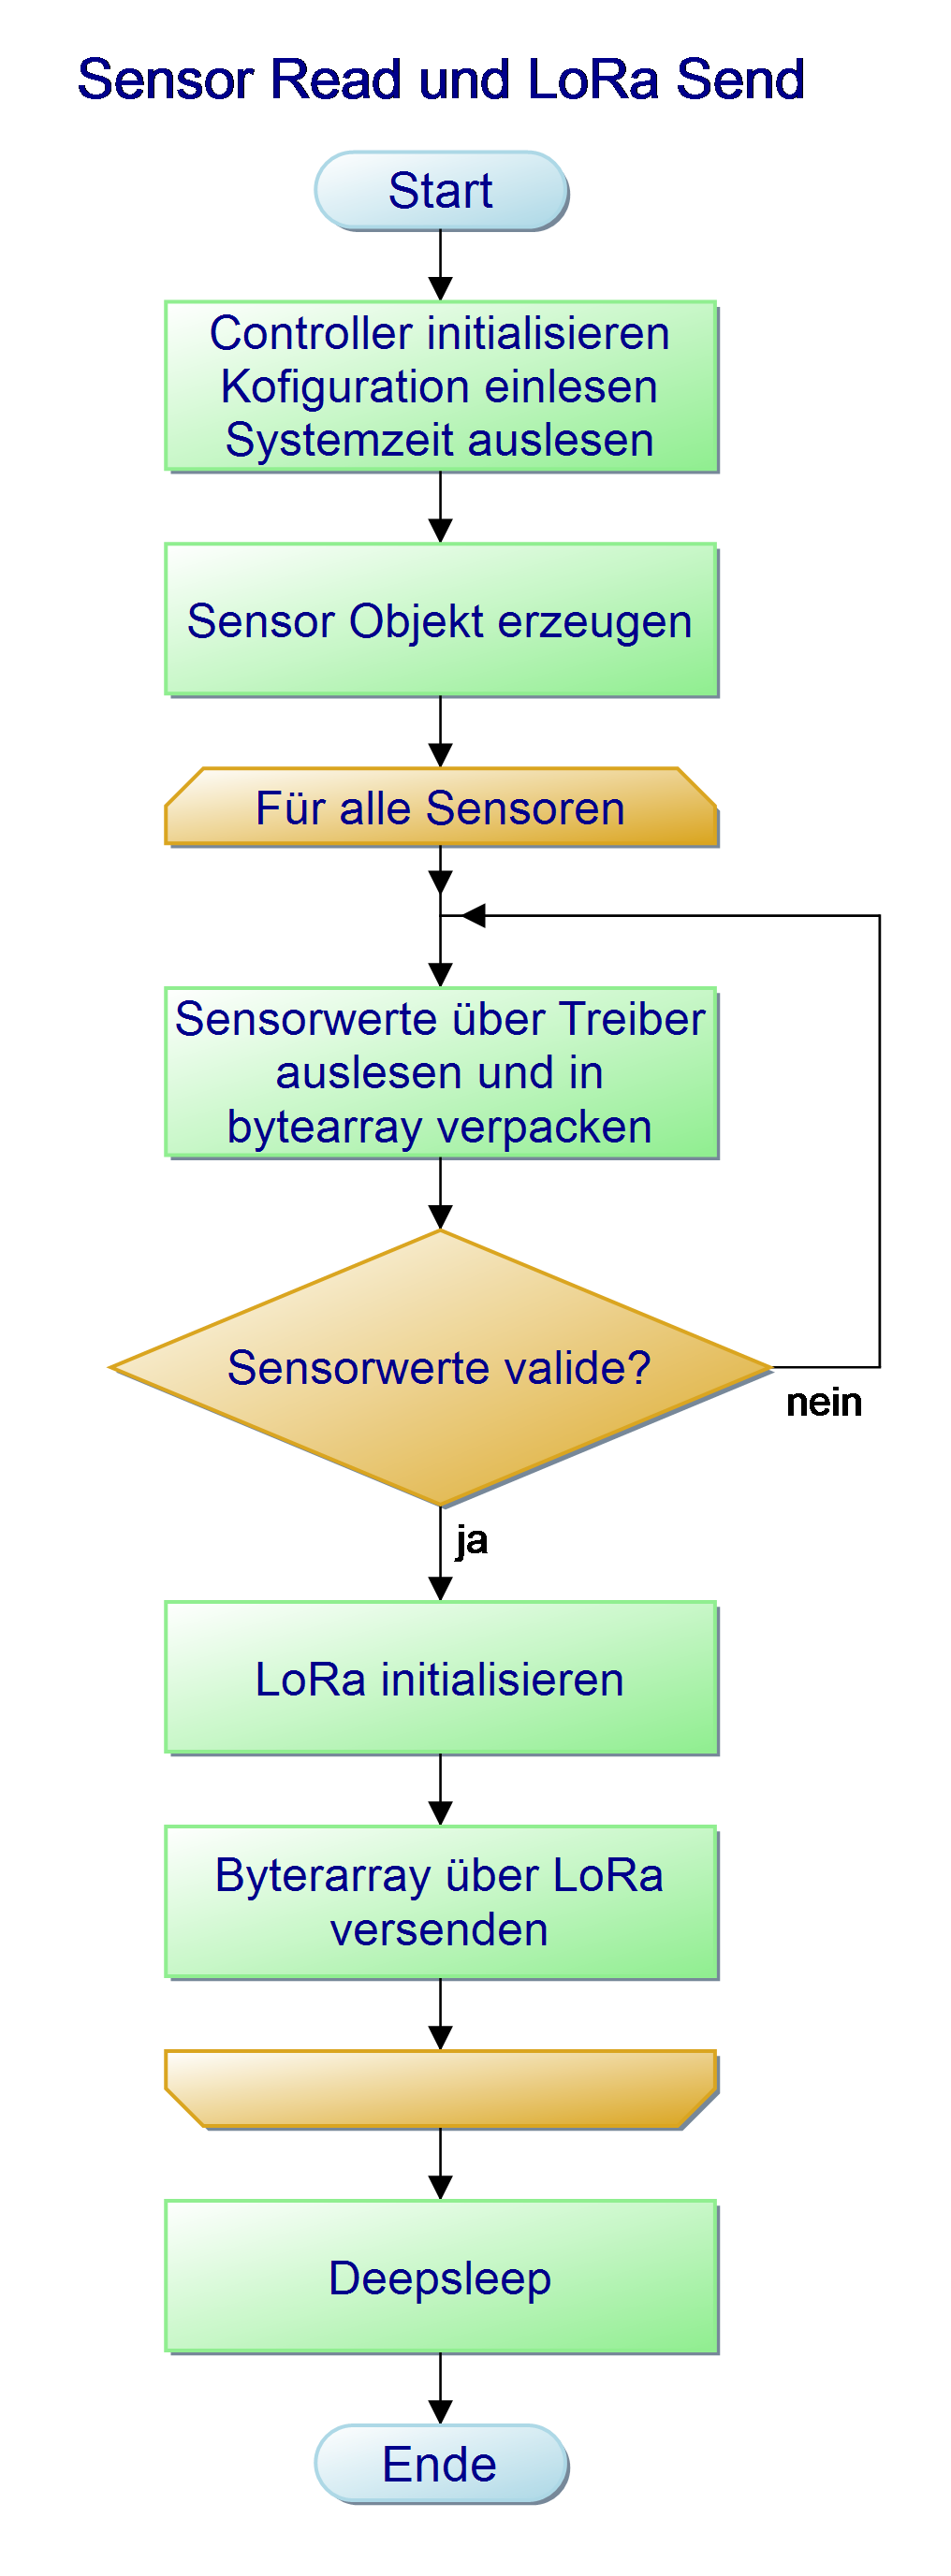
\includegraphics[width=0.4\textwidth]{pictures/sens_read_lora_send}}
	 \caption[PAP komponente 1]{Programm Ablauf: Komponente 1}
	 \label{fig:zeitplanung}
	\end{figure}
\end{center}

\subsection{2. Komponente: Emfangen der Daten und Versand ins Internet} \label{Empfänger}

\ldots

\subsection{3. Komponente: Manuelles abrufen und versenden der veröffentlichten Daten} \label{PubSub}

\ldots


\section{Visualisierung der Sensordaten} \label{Dashboard und Visualisierung}

\ldots


\section{Berechnung der Laufzeit im Batteriebetrieb} \label{Simulation}

\ldots
